\section{Mechanisms of Sintering}\label{sec:mechanisms}

The following elaborations on the basic theory of sintering are based on standard literature for the topic. Some notable textbooks are those of \textcite{German1996, German2014}, \textcite{Geguzin1973}, \textcite{Kang2005} and \textcite{Exner1978}.

This work concentrates on solid state sintering, meaning that there are only solid phases present in the system beside the surrounding atmosphere.
Liquid phase sintering, where the material partially melts to assist closing pores, is not regarded here.
Therefore, the term sintering shall always refer to solid state sintering from here on.

Sintering in general is a process, where powder material is densified and strengthened by thermal treatment at elevated temperatures.
The process is mainly driven by reduction of the energy stored in the system's microstructural features, such as grain boundaries, surfaces and other crystal defects.
The energy is dissipated as heat, so it is an irreversible process.
The microstructural state of the material is mainly transformed by diffusional flows to reach a state of lower energy.
In some systems, other transport mechanisms such as viscose or plastic flow can be observed, but are not regarded in the current work.

\begin{figure}
    \centering
    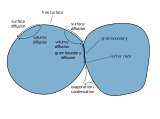
\includegraphics[width=\linewidth]{img/basic_theory/diffusion_mechanisms}
    \caption{Schematic Overview of Diffusion Mechanisms Observed in Sintering Processes}
    \label{fig:introduction/state_of_the_art/diffusion_mechanisms}
\end{figure}

In common sintering processes, the following diffusion mechanisms may occur.
Their importance depends on powder geometry, process conditions and material properties.
The place and usual direction of their occurrence is visualized in \cref{fig:introduction/state_of_the_art/diffusion_mechanisms}.

\begin{description}
    \item[Volume/Lattice Diffusion] is the diffusion of vacancies or interstitial atoms in the bulk material.
        It is usually one of the slowest mechanisms and often negligible.
    \item[Surface Diffusion] is the diffusion of mobile atoms on free surfaces (interfaces with surrounding atmosphere or vacuum).
        It is much faster than volume diffusion.
    \item[Grain Boundary Diffusion] is the diffusion of mobile atoms along grain boundaries (solid-solid interfaces).
        It is usually slower than surface diffusion but faster than volume diffusion.
        The effect of grain boundary diffusion compared to volume diffusion was paraphrased by \textcite{Fisher1951} with the heat flux in a foil of copper embedded in cork.
    \item[Evaporation and Condensation] is the evaporation of atoms, their diffusion through the gas phase and finally their condensation at another location.
        This mechanism features fast transport through the gas phase, but usually occurs only at very high temperatures, with very volatile substances or due to chemical reactions.
        The rate of evaporation is usually the rate determining mechanism.
\end{description}

Macroscopically these mechanisms can be observed via properties of the body such a size and shape or of the material such as strength, density, electrical and magnetic properties or chemical surface activity.

The most commonly observed effect is shrinkage, which means that the sintered body is smaller than the green body.
This is caused by transport of material from between the particles to the surface of the neck via grain boundary diffusion or volume diffusion.
Sole surface diffusion does not cause shrinkage.
As the mass of the system is constant, shrinkage must coincide with an increase in density, respectively a decrease of the amount of voids (porosity) in the body.
Shrinkage as a linear strain $\Shrinkage$ is usually quantified normed on the initial (green body) size $L_0$ as in \cref{eq:shrinkage}, where $L$ is the current size.
\begin{equation}
    \Shrinkage = \frac{L - L_0}{L_0}
    \label{eq:shrinkage}
\end{equation}

Most material properties are directly correlated with the size of the boundaries between the particles which form during sintering, called sinter necks.
The driving force for neck formation is the reduction of surface area in interaction with the energy stored in grain boundaries, where the latter is usually much smaller per area unit.
Most notably, the strength varies directly with the neck size, since the largest part of the load is transmitted via the necks, but also electric and magnetic properties.
The neck is usually measured in terms of its radius $\NeckRadius$ or cross-section area $\NeckArea$.

By the dominating mechanisms and their effect on neck growth and shrinkage, sintering is usually divided in three stages:

\begin{description}
    \item[Initial/Early Stage]
        The initial contact is created.
        Major diffusion occurs along surfaces to the sinter neck (triple points of surfaces and grain boundary).
        The neck size rapidly increases, but shrinkage is usually low.
    \item[Intermediate Stage]
        The porosity is still open and connected.
        Major diffusion occurs along the grain boundaries to the pores.
        The removal of substance at grain boundaries leads to large shrinkage.
    \item[Final/Late Stage]
        The porosity is mainly closed.
        The gas pressure in pores may affect sintering.
        There is still mainly grain boundary, but also volume diffusion.
        There is slow progress in shrinkage and densification.
\end{description}
